\documentclass[titlepage,11pt,a4paper]{article}
\usepackage[utf8]{inputenc}
\usepackage[french]{babel}
\usepackage{hyperref}
\usepackage{amsmath}
\usepackage{amsfonts}
\usepackage{amssymb}
\usepackage{stmaryrd}
\usepackage{polytechnique}
\usepackage{caption}
\usepackage{graphicx}
\usepackage{float} 
\usepackage{slashbox}
\usepackage{array}
\usepackage{enumitem}

\title[Projet INF552]{Reconstitution 3D et détection d’objets en milieu urbain}
\subtitle{Projet INF552 \\ Rapport Final}
\author{ Romain \textsc{LOISEAU}\\ Lucas \textsc{BROUX}}
\date{Pour le 8 Décembre 2017}
%\logo[headers]{Chemin relatif vers le logo}

\begin{document}
\maketitle

\newpage 

\newpage \tableofcontents

\newpage \section{Introduction}
% Contexte du projet.
\par Ce projet, réalisé dans le cadre du cours \emph{INF552 - Analyse d'Images et Vision par Ordinateur} consiste en l'analyse des images de la base de données \emph{Cityscapes} \href{(https://www.cityscapes-dataset.com/)}{(https://www.cityscapes-dataset.com/)} par les méthodes et algorithmes vus en cours. Cette base de données consiste en des images stéréo d'environnements urbains, prises par deux caméras installées sur le capot d'une voiture, dont on connait à tout instant les matrices. Les auteurs de la base de données fournissent les images prises par la caméra de gauche, la disparité calculée avec l'image de droite, ainsi que les informations géométriques des deux caméras.
% Objectifs du projet.
\par Notre objectif est le suivant : étant donnés une image de gauche, la disparité correspondante, ainsi que les données géométriques des deux caméras, reconnaitre des objets importants du paysages en n'utilisant que des algorithmes et méthodes étudiés en cours.
% Approche.
\par Notre approche est la suivante : dans un premier temps, nous utilisons ces informations pour reconstituer un nuage de point 3D correspondant à la prise de vue; puis nous appliquons l'algorithme RANSAC pour détecter le plan principal de ce nuage de points, le sol; enfin, nous avons développé plusieurs approches (RANSAC, \emph{clustering}) pour détecter les objets verticaux i.e. orthogonaux à ce plan.
% Plan du rapport.
\par Dans ce rapport, nous présentons tout d'abord notre approche et précisons les algorithmes employés. Nous présentons ensuite les résultats obtenus et analysons la performance de nos algorithmes. Enfin, nous concluons en présentant les enseignements acquis au cours de ce projet.
\par Le code source du projet est disponible sur ce repository github : \href{https://github.com/lucas-broux/Projet-Inf552}{https://github.com/lucas-broux/Projet-Inf552}



\newpage \section{Algorithmes utilisés et raisonnements}
\subsection{Reconstitution de nuage 3D}
% Reconstitution de nuage 3d à partir de l'image de gauche, la disparité, la matrice de la caméra.
\par Nous nous donnons l'image prise par l'appareil de gauche, marquée par les coordonnées $x$ et $y$, ainsi que l'image correspondant à la disparité $d \left( x, y \right)$, et les données géométriques des deux caméras i.e. leur paramètres intrinsèques et extrinsèques. 
\par Soit $X, Y$, et $Z$ les coordonnées 3D correspondant au point $x$, $y$ sur l'image de gauche, et $ d:=d\left(x, y\right)$. On note aussi $t$ la valeur de translation horizontale entre les deux caméras. Les équations de projection s'écrivent alors :
\begin{displaymath}
	\begin{split}
	\left\lbrace
	\begin{array}{cc}
	s * 
		\begin{bmatrix}
			x \\
			y \\
			1
		\end{bmatrix}
		 &=
		\begin{bmatrix}
			f_{x} & 0 & c_{x} \\
			0 & f_{y} & c_{y} \\
			0 & 0 & 1
		\end{bmatrix}
		\begin{bmatrix}
			1 & 0 & 0 & 0 \\
			0 & 1 & 0 & 0 \\
			0 & 0 & 1 & 0
		\end{bmatrix}
		\begin{bmatrix}
			X \\
			Y \\
			Z \\
			1
		\end{bmatrix}
		\\
	s * 
		\begin{bmatrix}
			x - d \\
			y \\
			1
		\end{bmatrix}
		 &=
		\begin{bmatrix}
			f_{x} & 0 & c_{x} \\
			0 & f_{y} & c_{y} \\
			0 & 0 & 1
		\end{bmatrix}
		\begin{bmatrix}
			1 & 0 & 0 & t \\
			0 & 1 & 0 & 0 \\
			0 & 0 & 1 & 0
		\end{bmatrix}
		\begin{bmatrix}
			X \\
			Y \\
			Z \\
			1
		\end{bmatrix}
	\end{array}\right.
	\end{split}
\end{displaymath}

à résoudre en $s, X, Y$, et $Z$. L'inversion du système donne : 
 \begin{displaymath}
	\begin{split}
		\begin{bmatrix}
			X \\
			Y \\
			Z
		\end{bmatrix}
		 &= - \dfrac{t}{d}
		\underbrace{
		\begin{bmatrix}
			1 & 0 & -c_{x} \\
			0 & \dfrac{f_{x}}{f_{y}} & \dfrac{-f_{x} c_{y}}{f_{y}} \\
			0 & 0 & f_{x}
		\end{bmatrix}}_{:=N}
		\begin{bmatrix}
			x \\
			y \\
			1
		\end{bmatrix}
	\end{split}
\end{displaymath}

Ainsi, le calcul des points 3D revient à une simple multiplication matricielle.


\subsection{Détection du sol}
% Application de l'algorithme RANSAC pour détecter le sol.
\par Pour détecter le sol, nous cherchons le plan principal du nuage de points 3D, à l'aide de l'algorithme RANSAC.

\par Cet algorithme consiste à tirer aléatoirement un grand nombre de fois trois points dans le nuage de points, puis de regarder combien de points sont dans le plan défini par ces trois points. A l'issue du processus, on retient le plan contenant le plus de points.

\par Nous avons besoin de deux paramètres : l'épaisseur d'un plan et le nombre d'itérations de l'algorithme.

\par L'épaisseur d'un plan est défini à partir d'une longueur caractéristique du nuage de point. En effet, nous pouvons essayer de calculer la distance moyenne entre deux points voisins afin d'obtenir une longueur caractéristique. Or calculer pour chaque point la distance à son plus proche voisin à une complexité en $n^2$ avec la structure de donnée que nous utilisons (Rappel : nous utilisons un vecteur de \emph{Vec3d} pour stocker notre nuage de point). Comme notre nuage de point à de l'ordre du million de point, le calcul exact de cette grandeur serait trop gourmand pour être exécuté en un temps raisonnable. Pour faire face à ce problème, nous tirons aléatoirement $1000$ points pour lesquels nous cherchons la plus petite distance avec $10000$ autres points tirés aléatoirement. Nous faisons donc de l'ordre de $1000 * 10 000 = 10 000 000$ d'opérations, ce qui est soutenable par la machine. En contrepartie, nous n'obtenons pas la grandeur désirée mais une approximation supérieur à cette grandeur qui suffira pour les besoins du projet. Dans l'algorithme, tout point qui sera à une distance inférieure à cette grandeur caractéristique du nuage de point du plan sera considéré comme appartenant au plan.

\par Le second paramètre à calculer est le nombre d'itérations suffisant. La \href{https://en.wikipedia.org/wiki/Random_sample_consensus}{page wikipédia suivante} explique comment calibrer ce paramètre à notre problème.

\par Désignons par $w$ la probabilité qu'un point appartienne au plan. Cette grandeur n'est en général pas connue, mais nous pouvons en donner une approximation. Dans notre cas, nous avons estimé que $w = 0.2$. Comme il faut $3$ points pour définir le plan, $1-w^3$ est la probabilité qu'au moins un point parmi ceux tirés n'appartienne pas au plan. En désignant par $p$ la probabilité de réussite de l'algorithme attendue et par $k$ le nombre d'itérations du modèle, nous en déduisons que $1-p = (1-w^3)^k$. Cela implique donc que :

$$k = \frac{\log{1-p}}{\log{(1-w^3)}}$$

\par Le paramètre entré par l'utilisateur est donc une probabilité de réussite de l'algorithme $p$. A cela nous ajoutons deux fois l'écart type de $k$ afin de s'assurer de la réussite de l'algorithme. Cet écart type vaut $\frac{\sqrt{1-w^3}}{w^3}$.

\subsection{Détection d'objets verticaux}
\par Nous proposons deux approches pour réaliser la détection des objets verticaux sur la route.

% Application d'une variante de l'algorithme RANSAC pour détecter les objets verticaux.
\subsubsection{Variante de l'algorithme RANSAC}
\par Notre première idée est d'appliquer l'algorithme RANSAC dans le but de rechercher des lignes dans l'espace; en ajoutant une contrainte sur leur verticalité. Pour cela, nous utilisons le même algorithme que précédemment en l'adaptant aux lignes. De plus, nous recherchons plusieurs lignes. De plus, nous ajoutons une contrainte sur la verticalité des lignes détectées en s'assurant que l'angle entre la normale au plan de la route et la direction de la ligne trouvée soit inférieur à une constante fixée au préalable.

\par Cette méthode est assez mauvaise dans la détection des objets verticaux. En effet, dans le nuage de points on ne distingue pas vraiment de lignes, et il semble donc compliqué pour notre algorithme de fonctionner efficacement sur ce type de données.

% Application d'un algorithme de clustering.
\subsubsection{Algorithme des k-moyennes}
\par Notre seconde approche est fondée sur l'algorithme des k-moyennes. Nous commençons par choisir $k$ centres de \emph{clusters} aléatoirement dans le nuage de point. Ensuite nous calculons les \emph{clusters} en assignant chaque point au barycentre dont il est le plus proche. Nous itérons ensuite jusqu'à ce que le modèle converge. Voici les quelques spécificités de notre algorithme :

\begin{itemize}
\item{Le nombre d'itérations est calculé de telle sorte que l'algorithme s'arrête lorsque les barycentres se stabilisent. Dans notre cas, lorsque la variation de la variation de barycentre moyenne est inférieure à $1\%$  de la variation de barycentre moyenne du pas précédent. Pour éviter toutefois de boucler indéfiniment, nous avons ajouté un seuil à ne pas dépasser pour le nombre d'itérations.}
\item{Nous changeons également la topologie de l'espace des positions. En effet, les objets que nous souhaitons détecter sont des objets verticaux. Ils sont donc par nature étirés selon l'altitude. Pour que l'algorithme les détecte plus facilement, nous comprimons l'axe vertical afin de rapprocher les points selon cet axe. Ainsi, cela revient à avoir un algorithme qui regarde le nuage de points du ciel. Cela se fait en deux étapes. Tout d'abord, nous faisons un changement de base en fixant l'axe vertical du monde réel comme égal au vecteur normal au plan trouvé précédemment. Ensuite, nous utilisons trois variables constantes spécifiant le degré de compression selon chacun des axes.
\begin{itemize}
\item{const double $SCALER_X = 0.5$;}
\item{const double $SCALER_Y =1$;}
\item{const double $SCALER_Z = 1$;}
\end{itemize}
Ainsi, à chaque calcul de distance, nous multiplierons chacune des dimensions par le coefficient adéquat}
\item{Enfin, nous avons la possibilité d'utiliser l'algorithme en prenant en entrée la couleur de chacun des points. Cela nous permet de prendre en compte le fait que lorsqu'on veut détecter un objet vertical, on a de bonnes raisons de penser que sa couleur va être homogène. Ainsi, nous pouvons réaliser l'algorithme en utilisant non plus trois dimensions, mais six. Nous commençons donc par définir un paramètre permettant de définir l'importance de la couleur dans l'algorithme. A l'image des trois paramètres utilisés précédemment, cela permet de changer la topologie de l'espace pour donner plus ou moins d'importance à la couleur. Nous utilisons ensuite ce paramètre en le définissant comme le produit de deux termes
\begin{itemize}
\item{Le rapport de l'écart-type en position et de l'écart-type en couleur. Cela permet de procéder à une normalisation des couleurs par rapport aux positions. En effet, il n'y a pas de raison que les valeurs de position et de couleurs évoluent dans le mêmes ordres de grandeur.}
\item{Un paramètre ressemblant aux paramètres nommés précédemment qui permet de donner arbitrairement plus ou moins d'importance à la couleur dans le calcul des k-moyennes.}
\end{itemize}}
\item{Le score que nous utilisons pour évaluer la performance est un score nommé \emph{silhouette score}. Il permet de s'assurer que l'algorithme cherche le bon nombre de \emph{clusters}. Il s'intéresse à la différence entre la distance d'un point à son \emph{cluster} et la distance du même point au \emph{cluster} le plus proche dont il ne fait pas partie.}
\end{itemize}

\newpage \section{Résultats, performance, perspectives d'amélioration}
\subsection{Exemples de résultats}
% Donner des exemples de résultats :
%	- Point cloud.
%	- Détection du sol.
%	- Détection des objets verticaux.
\par Voici quelques visualisations des résultats obtenus :
\subsubsection{Nuage de points 3D}
\begin{figure}[H]
  \centering
%  \hspace*{-1cm}
    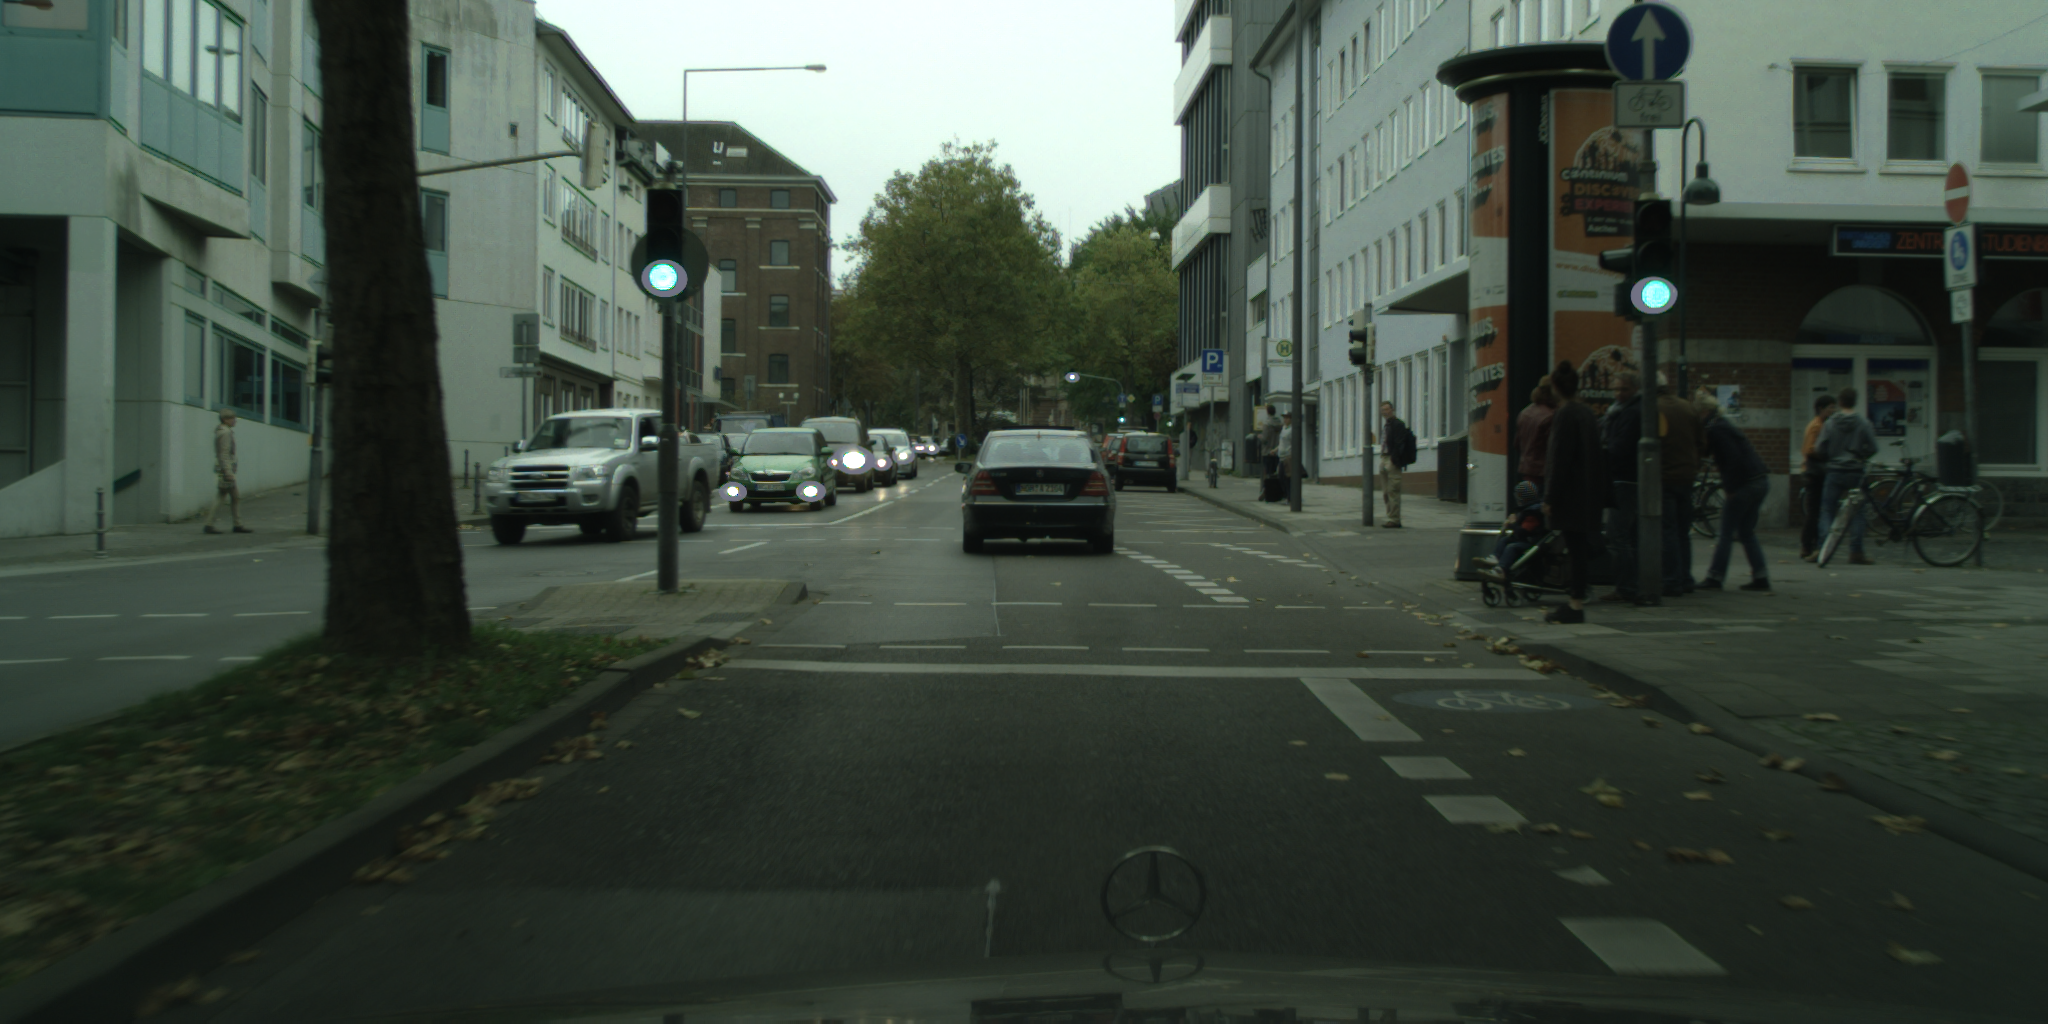
\includegraphics[width=0.45\textwidth]{images/aachen_000029_000019_leftImg8bit.png}
  \hfill{}
    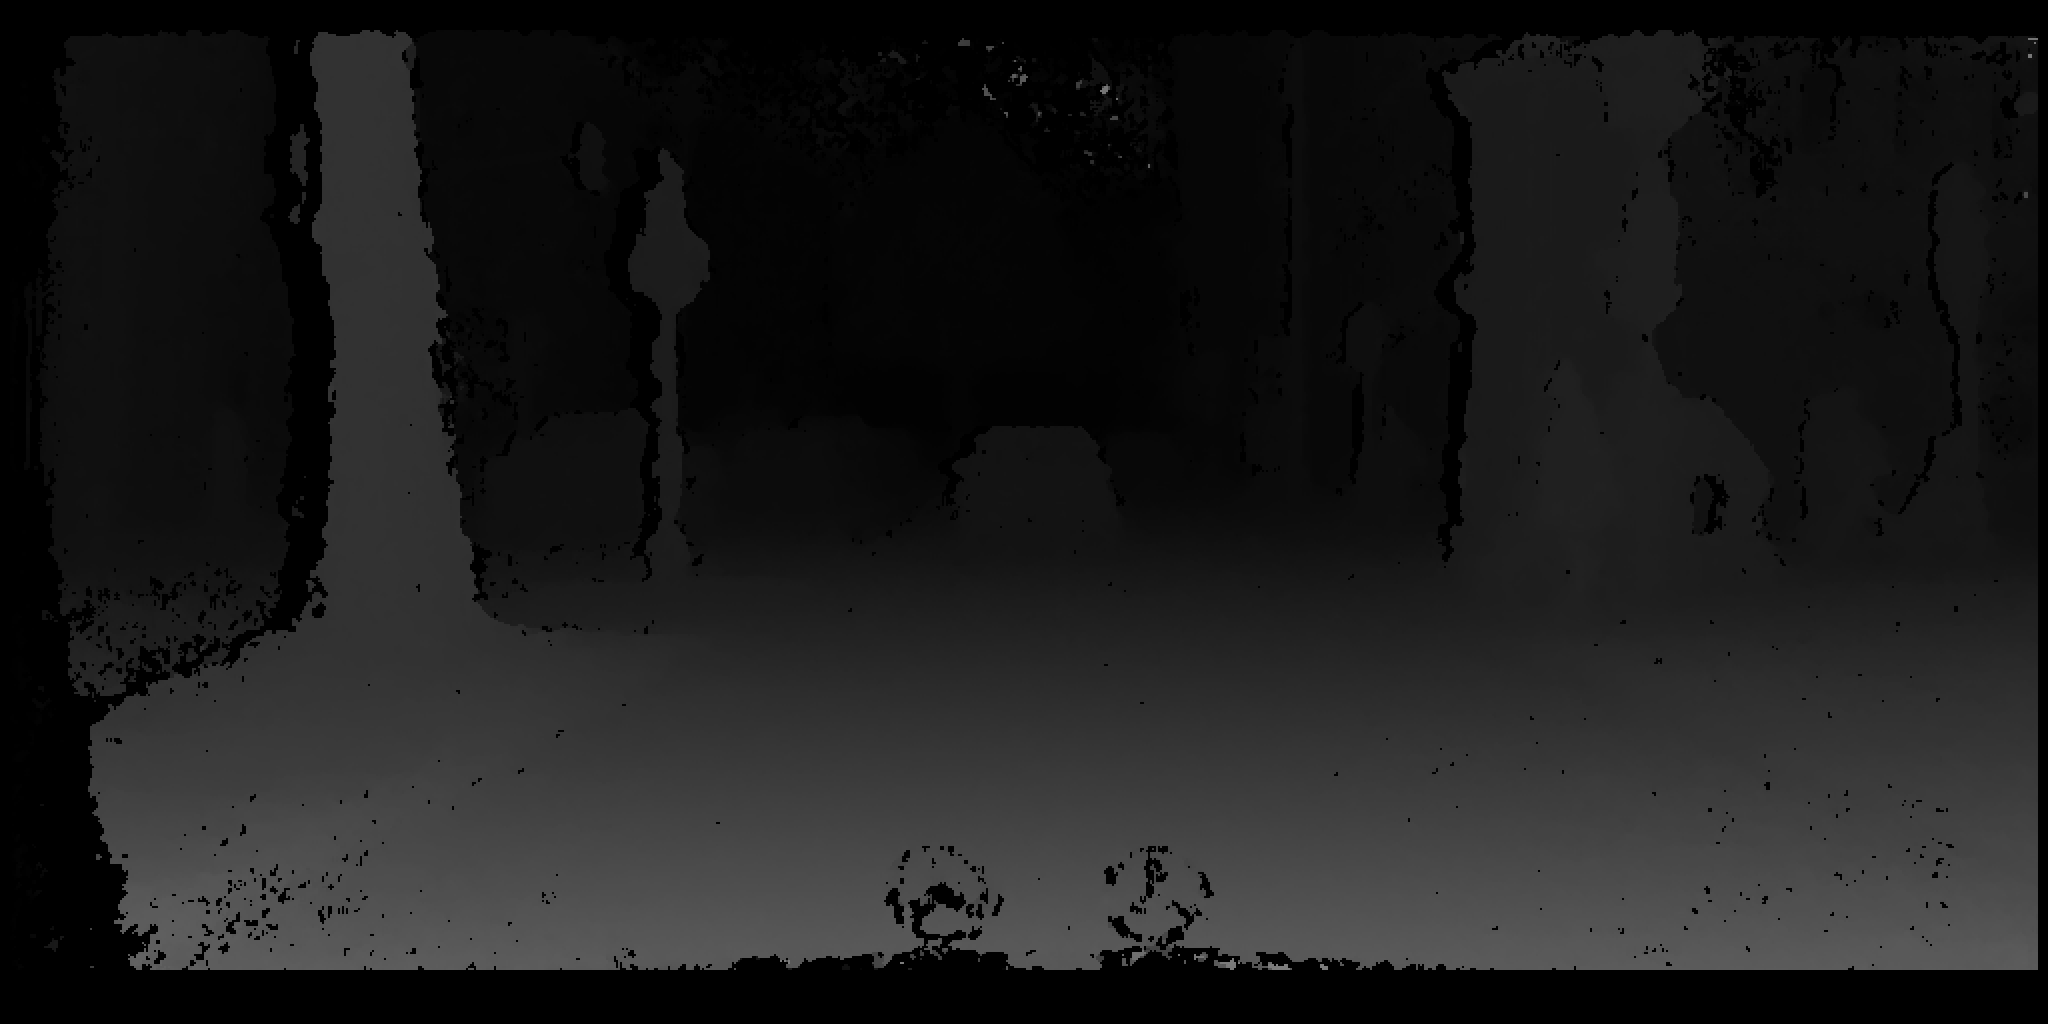
\includegraphics[width=0.45\textwidth]{images/aachen_000029_000019_disparity.png}
  \hfill 
  \caption{Image d'origine et sa disparité}
\end{figure} 
\begin{figure}[H]
  \centering
%  \hspace*{-1cm}
    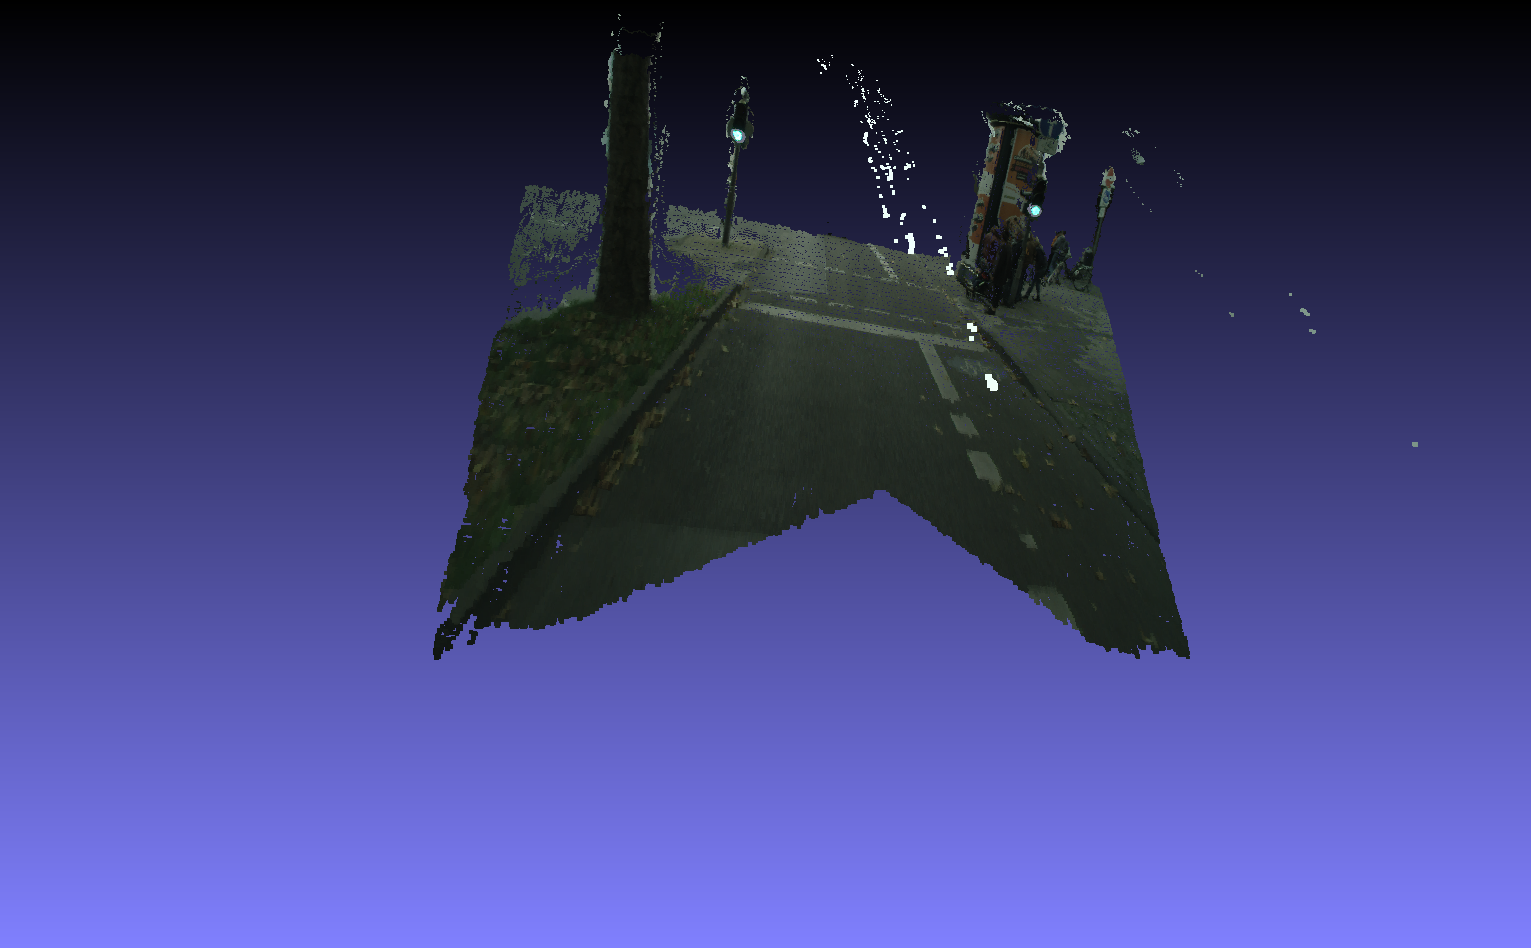
\includegraphics[width=0.45\textwidth]{images/3dpointcloud00.png}
  \hfill{}
    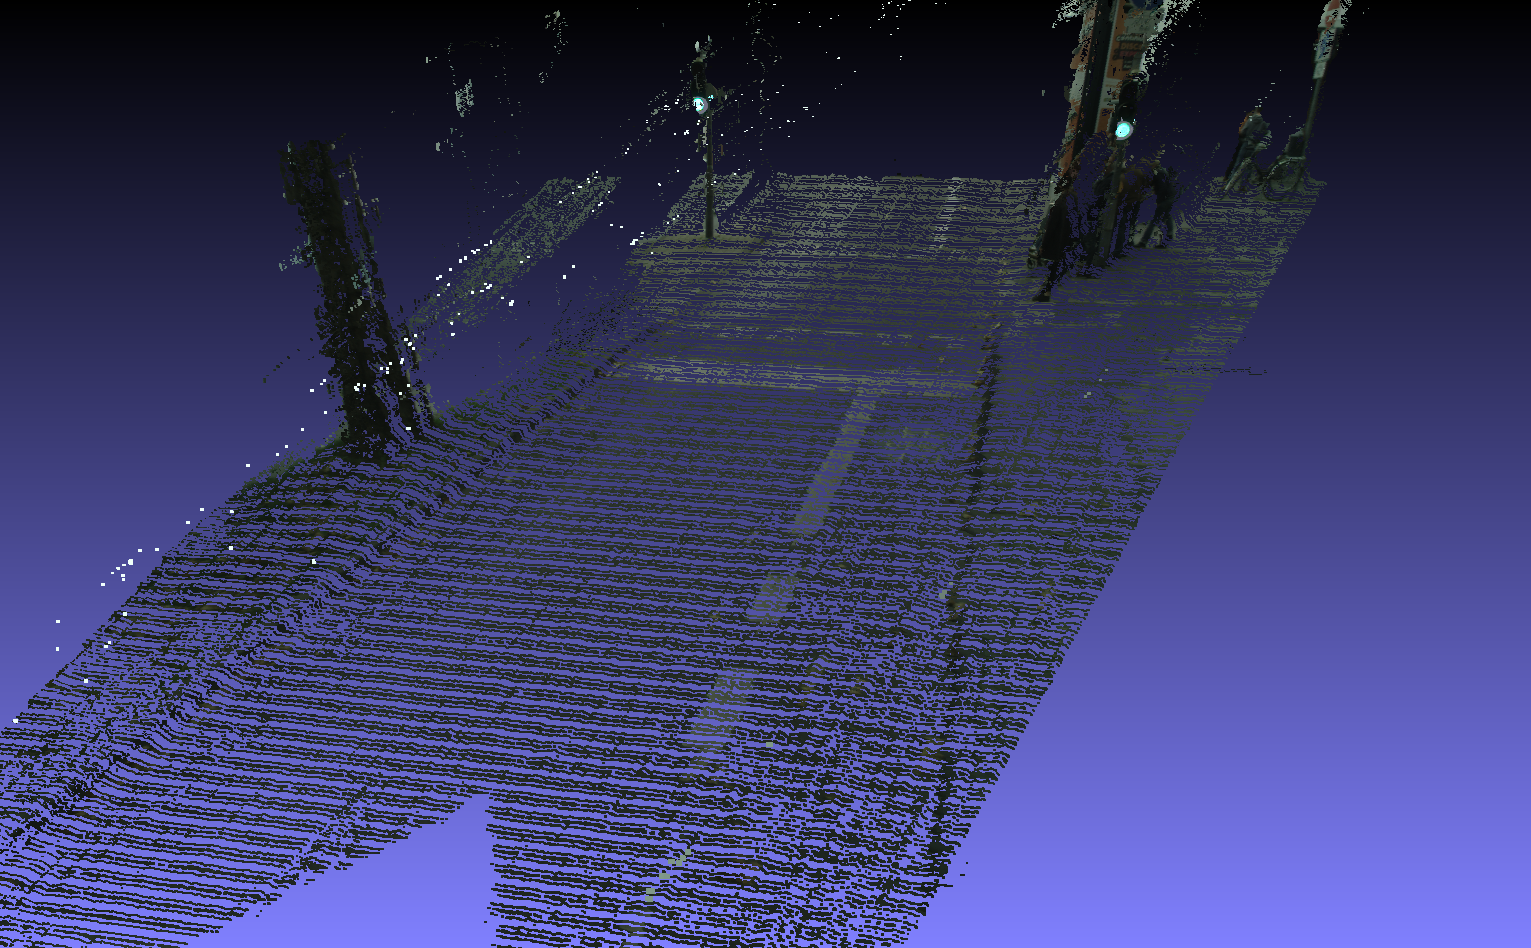
\includegraphics[width=0.45\textwidth]{images/3dpointcloud01.png}
  \hfill 
  \caption{Nuage de point 3d obtenu (Visualisation sur MeshLab)}
\end{figure} 

\subsubsection{Détection de la route et des éléments verticaux par RANSAC}
\par Voilà les résultats obtenus sur une dizaine d'images pour notre implémentation de l'algorithme de RANSAC. Nous représentons en rouge la route, en vert les éléments verticaux.

\begin{figure}[H]
  \centering
%  \hspace*{-1cm}
    \includegraphics[width=0.45\textwidth]{images/result_ransac/result_0.jpg}
  \hfill{}
    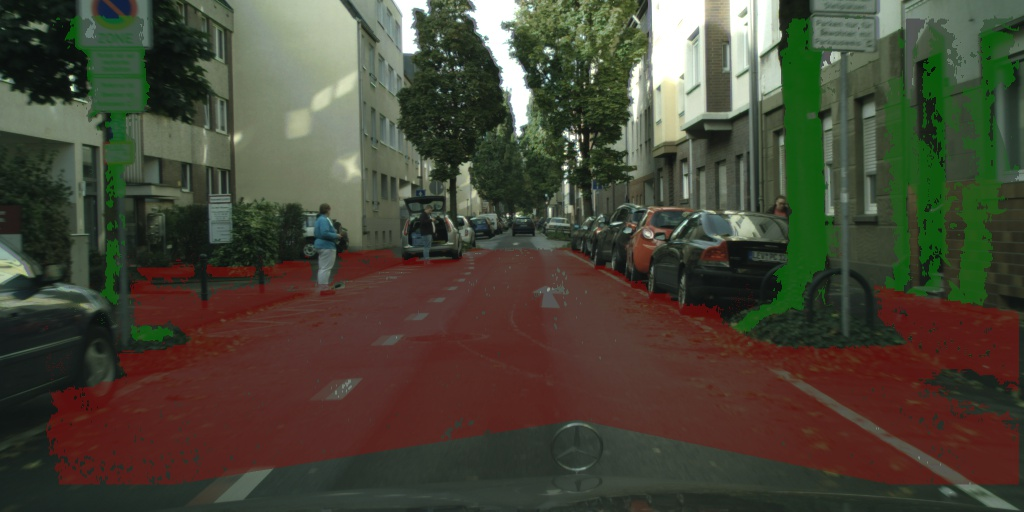
\includegraphics[width=0.45\textwidth]{images/result_ransac/result_1.jpg}
  \hfill 
  \caption{Algorithme RANSAC}
\end{figure} 
\begin{figure}[H]
  \centering
%  \hspace*{-1cm}
    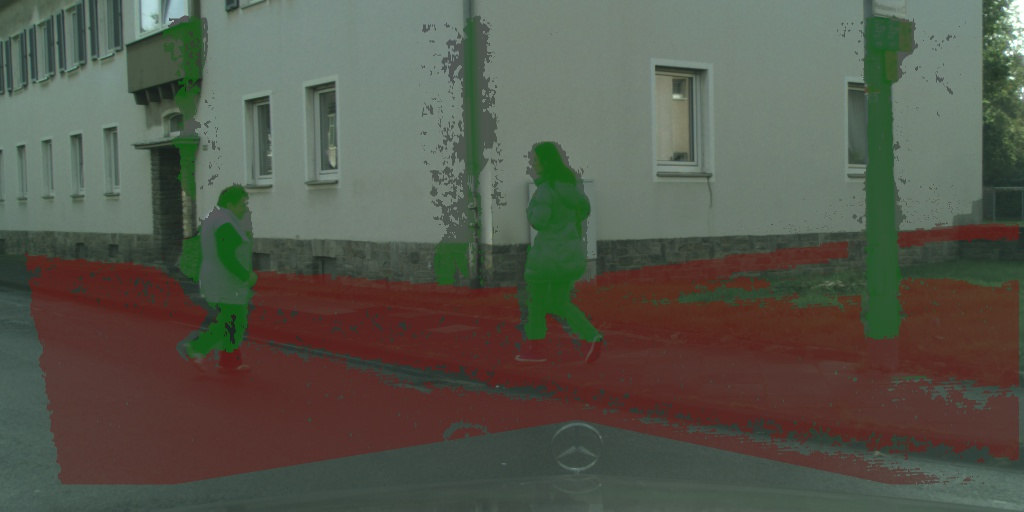
\includegraphics[width=0.45\textwidth]{images/result_ransac/result_2.jpg}
  \hfill{}
    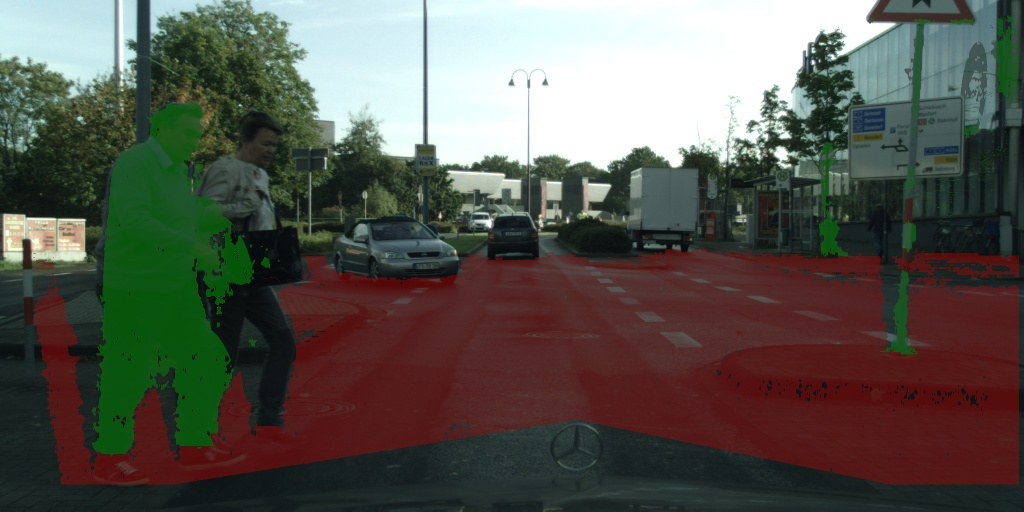
\includegraphics[width=0.45\textwidth]{images/result_ransac/result_3.jpg}
  \hfill 
  \caption{Algorithme RANSAC}
\end{figure} 
\begin{figure}[H]
  \centering
%  \hspace*{-1cm}
    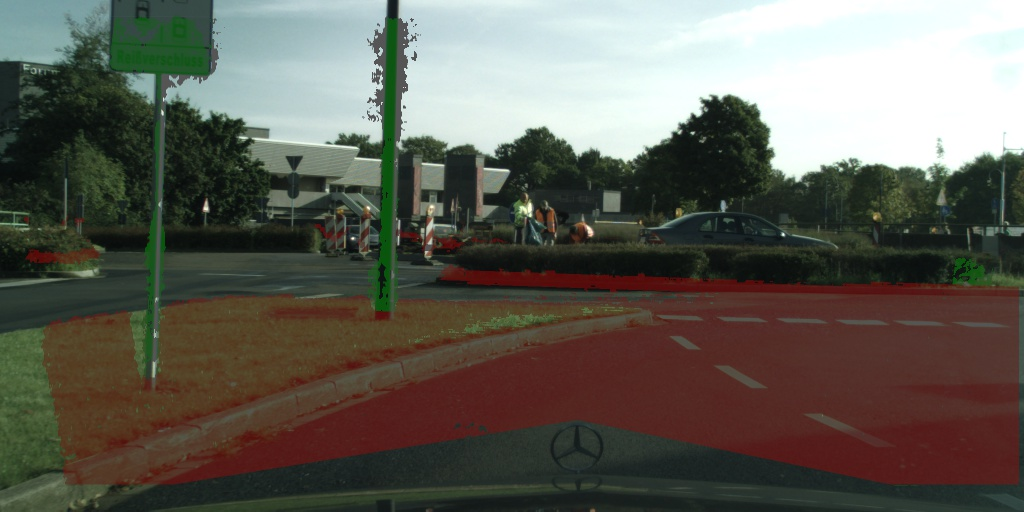
\includegraphics[width=0.45\textwidth]{images/result_ransac/result_4.jpg}
  \hfill{}
    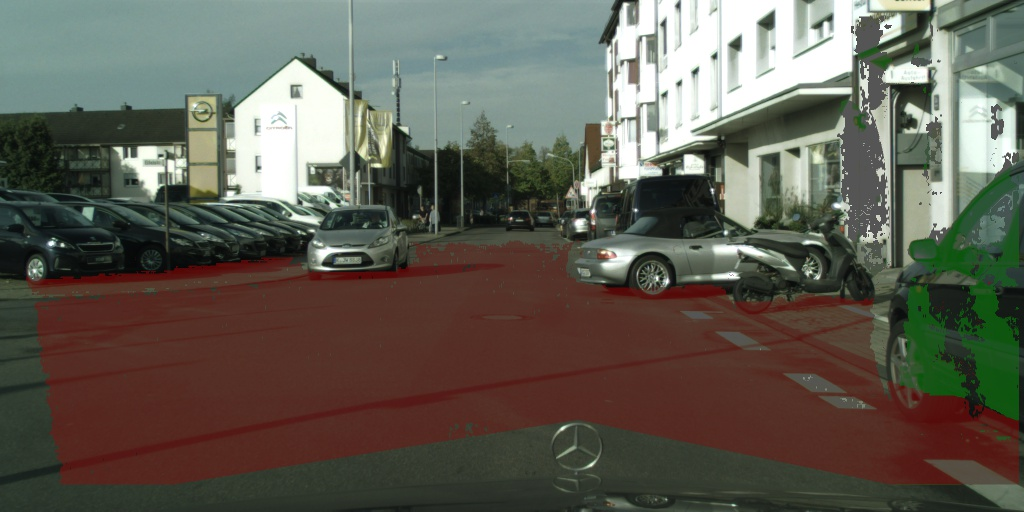
\includegraphics[width=0.45\textwidth]{images/result_ransac/result_5.jpg}
  \hfill 
  \caption{Algorithme RANSAC}
\end{figure} 
\begin{figure}[H]
  \centering
%  \hspace*{-1cm}
    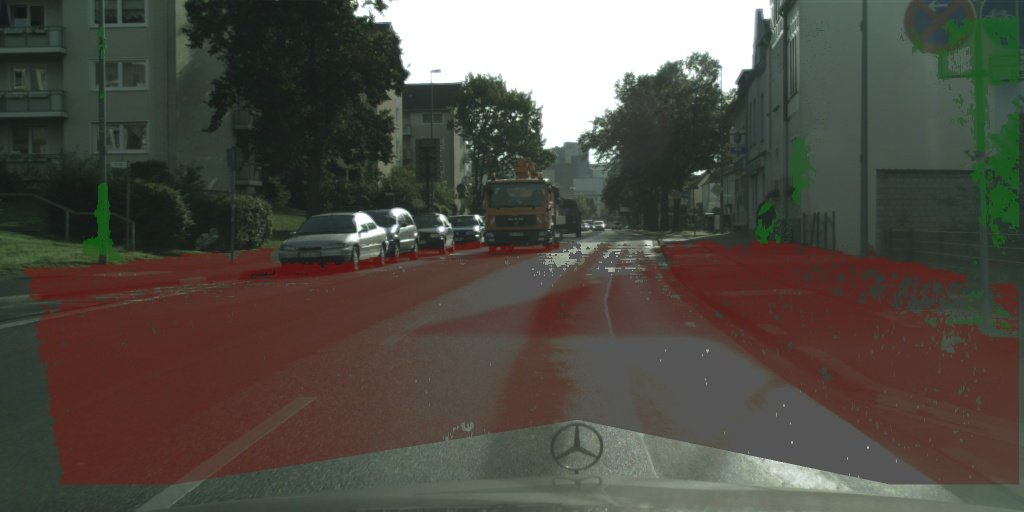
\includegraphics[width=0.45\textwidth]{images/result_ransac/result_6.jpg}
  \hfill{}
    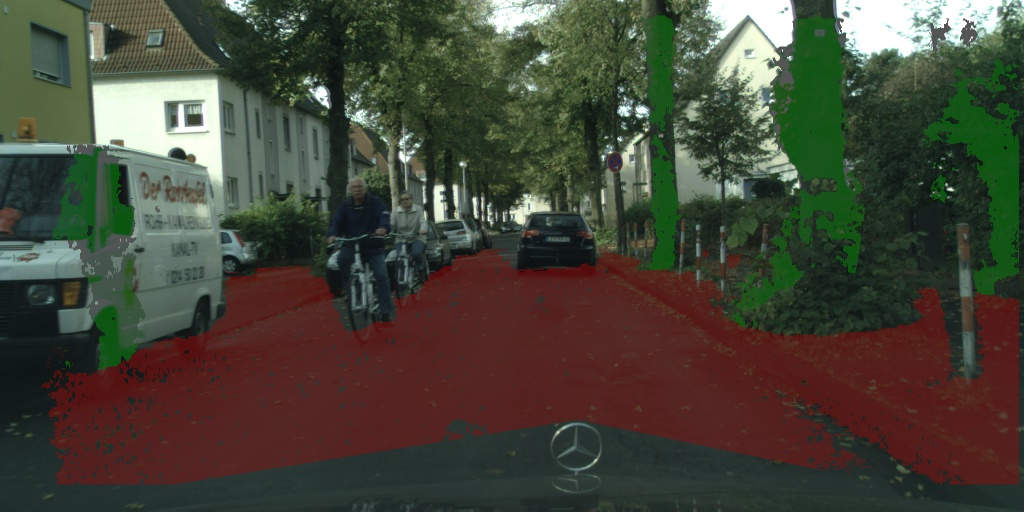
\includegraphics[width=0.45\textwidth]{images/result_ransac/result_7.jpg}
  \hfill 
  \caption{Algorithme RANSAC}
\end{figure} 
\begin{figure}[H]
  \centering
%  \hspace*{-1cm}
    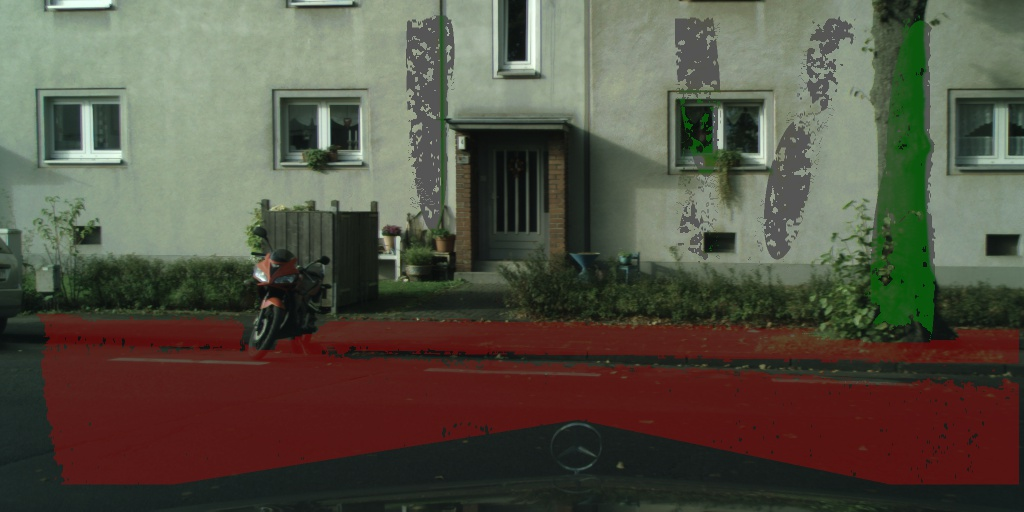
\includegraphics[width=0.45\textwidth]{images/result_ransac/result_8.jpg}
  \hfill{}
    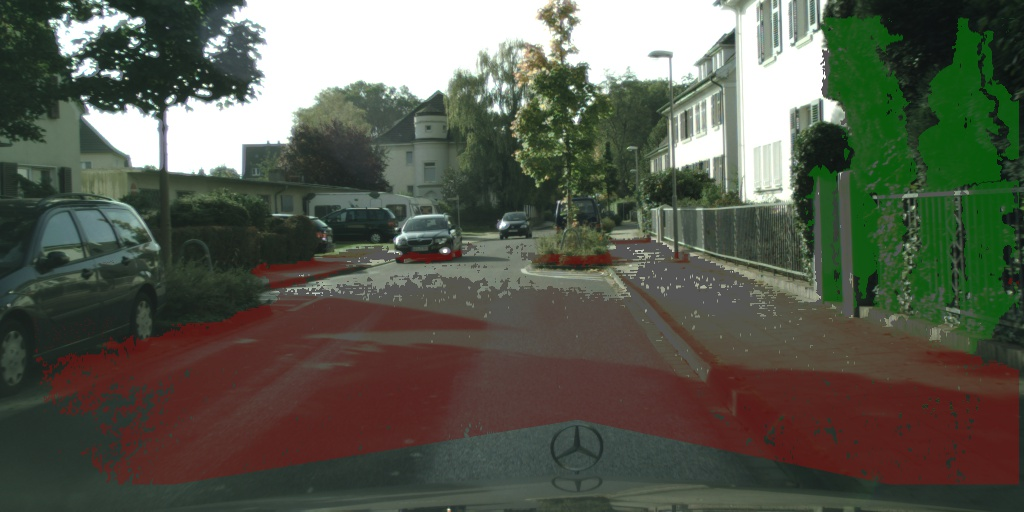
\includegraphics[width=0.45\textwidth]{images/result_ransac/result_9.jpg}
  \hfill 
  \caption{Algorithme RANSAC}
\end{figure}

\par Nous remarquons que l'algorithme de détection de la route est très précis, retournant le plan correct sur chacune des images.
\par En revanche, si nous constatons que l'algorithme est efficace pour repérer les éléments verticaux (poteaux, passants, arbres, ...), il ne permet pas de distinguer certains objets plus aplatis ou plans (voitures, murs, ...) et renvoie des résultats aberrants dans le cas ou aucun objet vertical n'est présent sur l'image.
Cela est du au fait que notre algorithme est conçu pour renvoyer un nombre fixe de lignes verticales.

\subsubsection{Détection d'objets par clustering}
\par Voilà les résultats obtenus sur une dizaine d'images pour notre algorithme de \emph{clustering}.

\begin{figure}[H]
  \centering
%  \hspace*{-1cm}
    \includegraphics[width=0.45\textwidth]{images/result_clustering/result_0.jpg}
  \hfill{}
    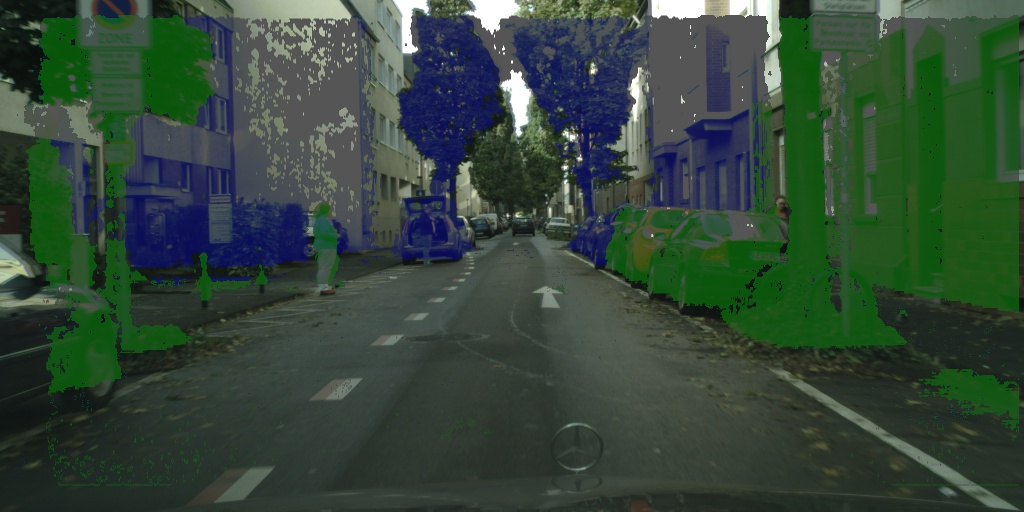
\includegraphics[width=0.45\textwidth]{images/result_clustering/result_1.jpg}
  \hfill 
  \caption{Algorithme des k-moyennes}
\end{figure} 
\begin{figure}[H]
  \centering
%  \hspace*{-1cm}
    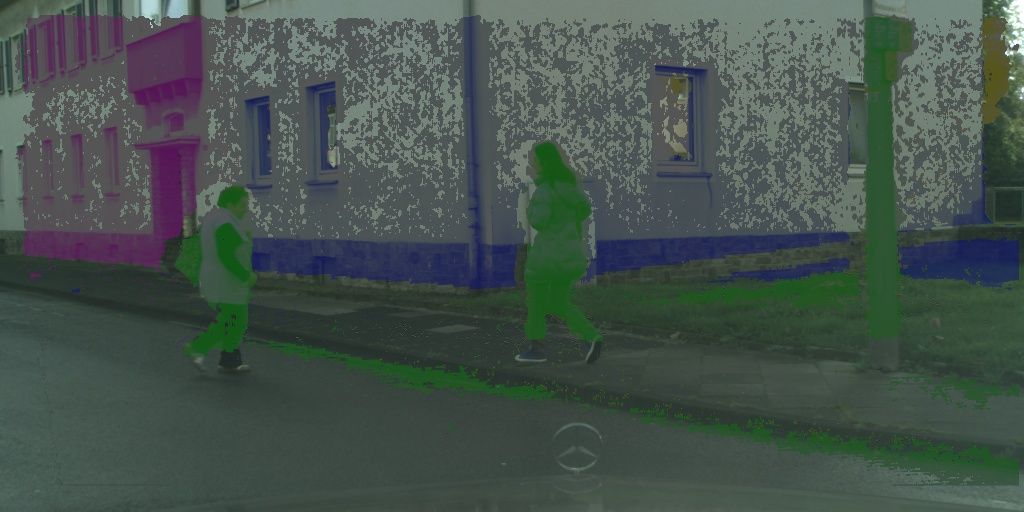
\includegraphics[width=0.45\textwidth]{images/result_clustering/result_2.jpg}
  \hfill{}
    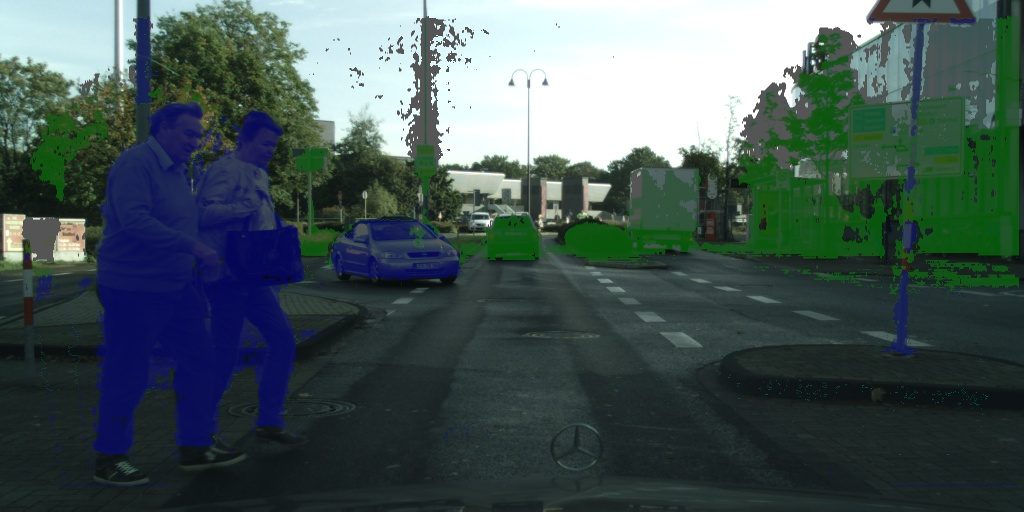
\includegraphics[width=0.45\textwidth]{images/result_clustering/result_3.jpg}
  \hfill 
  \caption{Algorithme des k-moyennes}
\end{figure} 
\begin{figure}[H]
  \centering
%  \hspace*{-1cm}
    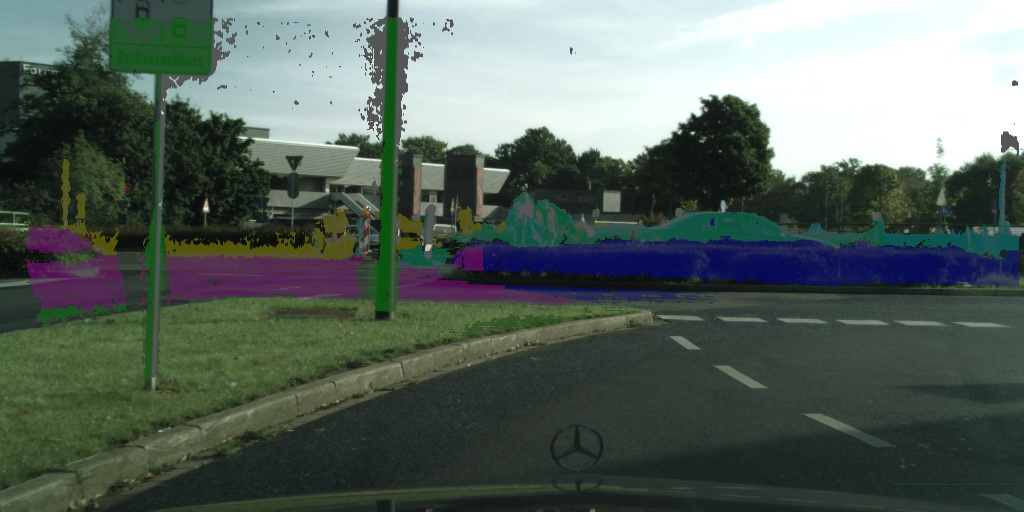
\includegraphics[width=0.45\textwidth]{images/result_clustering/result_4.jpg}
  \hfill{}
    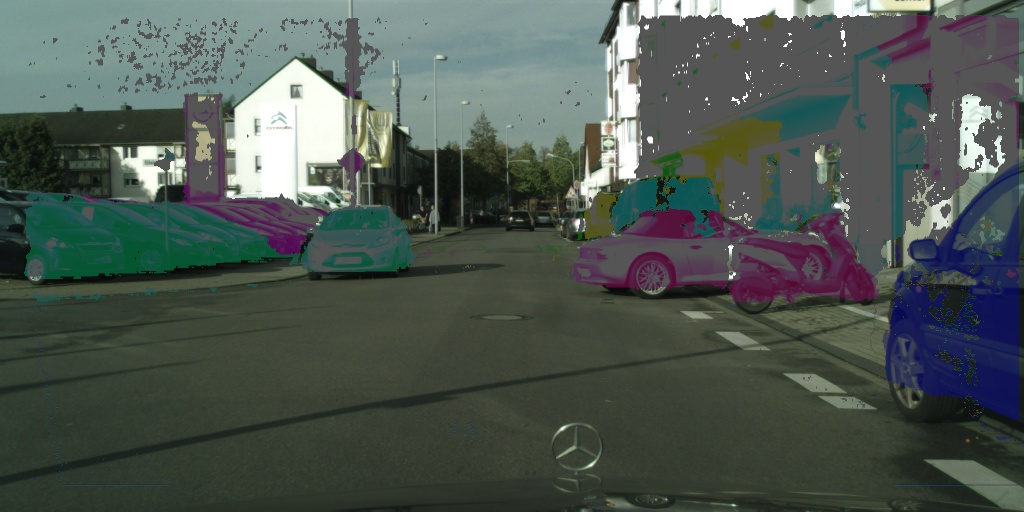
\includegraphics[width=0.45\textwidth]{images/result_clustering/result_5.jpg}
  \hfill 
  \caption{Algorithme des k-moyennes}
\end{figure} 
\begin{figure}[H]
  \centering
%  \hspace*{-1cm}
    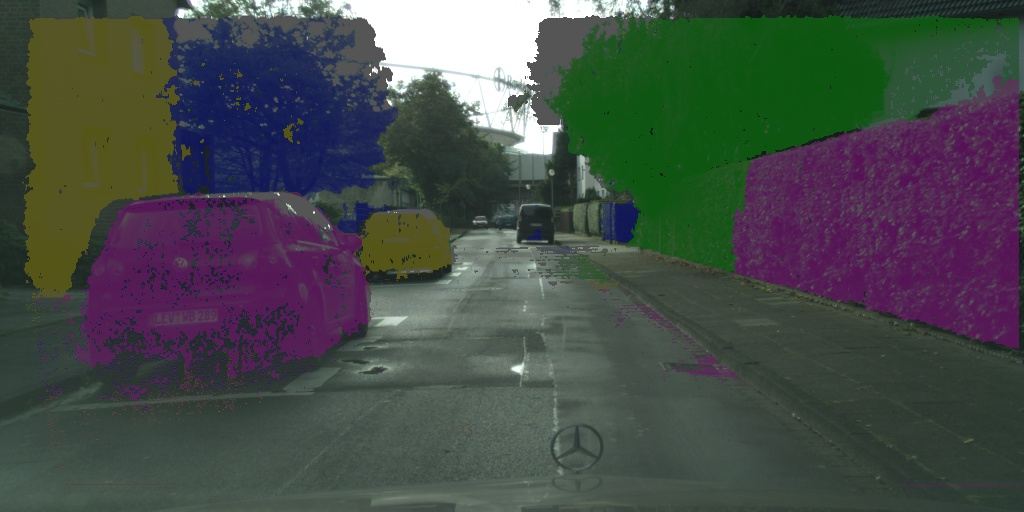
\includegraphics[width=0.45\textwidth]{images/result_clustering/result_6.jpg}
  \hfill{}
    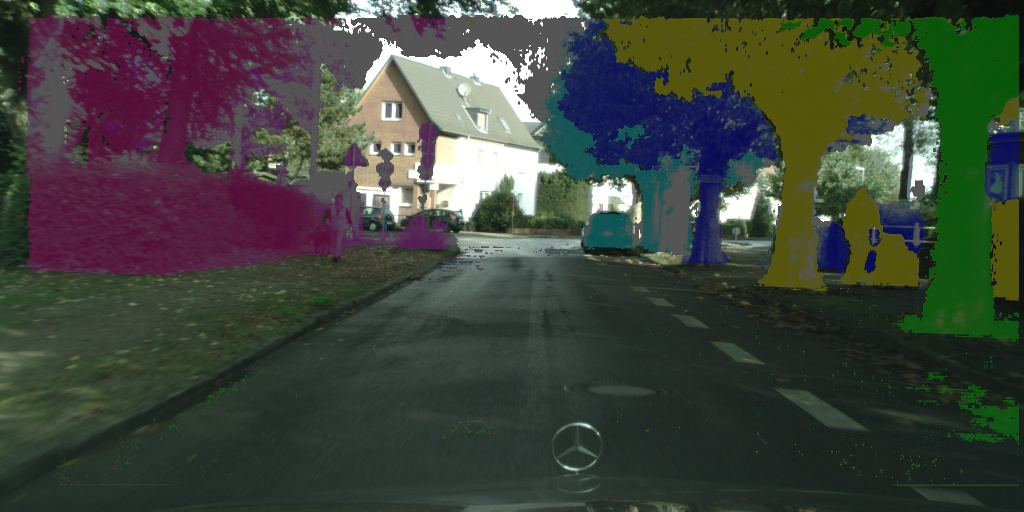
\includegraphics[width=0.45\textwidth]{images/result_clustering/result_7.jpg}
  \hfill 
  \caption{Algorithme des k-moyennes}
\end{figure}

\par Nos résultats sont mitigés. Les \emph{clusters} renvoyés par l'algorithme sont constitués en réalité de pans de l'espace agglomérés ensemble, et comportent parfois de nombreux objets distincts ou coupent ces objets en deux. Nous pensons que cela est dû à plusieurs facteurs : 
\begin{itemize}
\item D'une part, les algorithmes mis en œuvre reposent sur un certain nombre d'hyperparamètres qu'il faudrait analyser plus en détail pour pouvoir en comprendre l'impact et optimiser l'algorithme.
\item En outre, l'algorithme choisi pour réaliser le \emph{clustering} (algorithme des k-moyennes) est relativement basique et possède les inconvénients suivants vis à vis de nos données : 
	\begin{itemize}
	\item Il est basé sur l'hypothèse principale selon laquelle les \emph{clusters} à trouver sont globulaires, ce qui a pour effet de couper en plusieurs parties certains \emph{clusters} naturels qui ne le sont pas (haies, arbres, ...).
	\item Il prend en paramètre le nombre voulu de \emph{clusters}, qui n'est pas facile à estimer. Pour pallier ce problème, nous appliquons plusieurs fois l'algorithme en faisant varier la valeur de ce paramètre et nous appliquons un score (lui aussi assez simple) pour quantifier la pertinence du \emph{clustering}. Toutefois ce procédé contribue à une forte augmentation du temps de calcul.
	\item Enfin, l'algorithme ne prend pas en compte le bruit dans les données du problème, qui est pourtant bien présent à cause des légère imperfections dans les images de disparité fournies par le \emph{cityscapes dataset}. 
	\end{itemize}
	Nous pensons que d'autres algorithmes que nous n'avons pas pu implémenter pour des raisons de temps - par exemple l'algorithme DBSCAN, qui résout les 3 inconvénients ci-dessus - pourraient être plus efficaces et précis.
\end{itemize}


\subsection{Analyse de la performance}
% Évaluer la performance temporelle.
\par Pour juger la performance temporelle de nos algorithmes, nous avons réalisé une plateforme de tests, que nous avons appliquée à 57 images, sur un ordinateur portable standard.
\par Voici les histogrammes des temps de calcul des différents algorithmes employés : 
\begin{figure}[H]
  \centering
    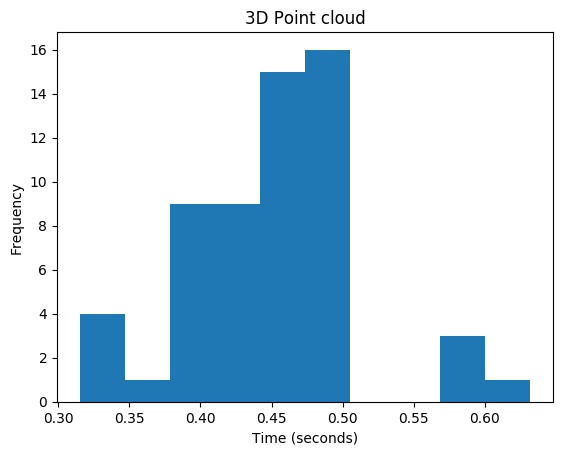
\includegraphics[width=0.7\textwidth]{images/3D_Point_cloud.png}
  \caption{Temps de calcul du nuage de points 3d}
\end{figure}

\par Nous constatons que le calcul du nuage de points 3D est relativement rapide (moins d'une demi-seconde quasiment systématiquement), en particulier étant donné le nombre de sommets calculés, qui est de l'ordre du million.


\begin{figure}[H]
  \centering
    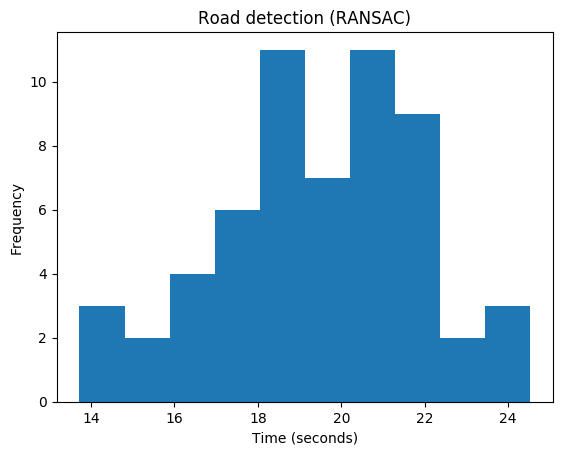
\includegraphics[width=0.7\textwidth]{images/Road_detection_(RANSAC).png}
  \caption{Temps de calcul pour la détection de la route}
\end{figure}

\par L'application de l'algorithme RANSAC pour la détection de la route est ainsi particulièrement long (de l'ordre de 20 secondes en moyenne). C'est donc une opération limitante d'un point de vue temporel.


\begin{figure}[H]
  \centering
    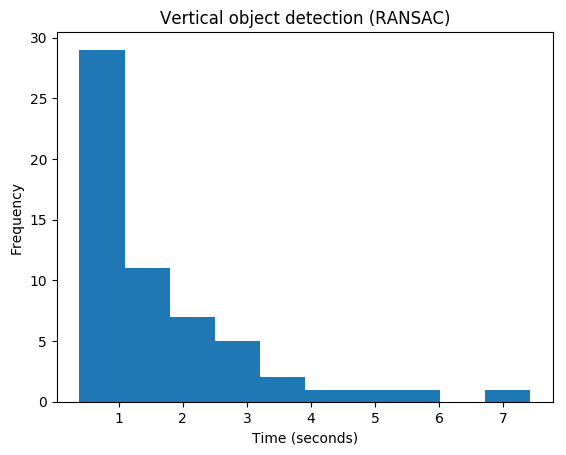
\includegraphics[width=0.7\textwidth]{images/Vertical_object_detection_(RANSAC).png}
  \caption{Temps de calcul pour la détection des objets verticaux (RANSAC)}
\end{figure}

\par Pour la détection des objets verticaux, l'algorithme RANSAC est donc relativement efficace, mais tout de même de l'ordre de plusieurs secondes en moyenne. 

\begin{figure}[H]
  \centering
    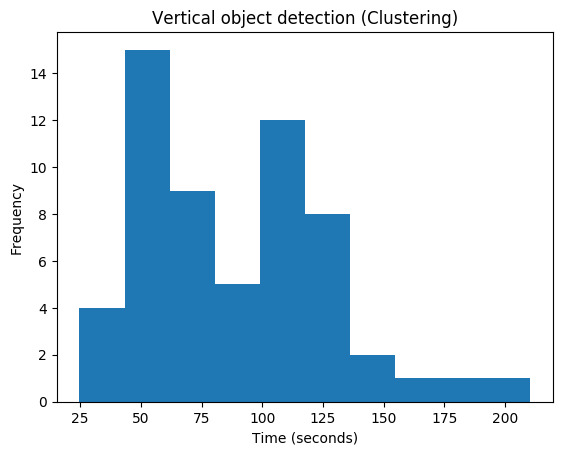
\includegraphics[width=0.7\textwidth]{images/Vertical_object_detection_(Clustering).png}
  \caption{Temps de calcul pour la détection des objets verticaux (k-moyennes)}
\end{figure}

\par Nous constatons que l'algorithme de \emph{clustering} choisi est particulièrement lent. Comme présenté précédemment, ceci est en partie dû au fait que nous l'appliquons plusieurs fois pour trouver le nombre optimal de \emph{clusters}, sachant que les données à analyser sont assez nombreuses ($\sim$ 1 million de points). Cela est peut-être aussi dû à nos choix d'implémentation : des structures de données plus efficaces et une meilleure prise en compte des possibilités d'optimisation du compilateur pourraient sûrement améliorer cette performance.


\subsection{Perspectives d'amélioration}
% Optimisation du code (écrit avec une connaissance assez limité des possibilités d'optimisation du compilateur, structures de données, ...).
% Choix des algorithmes et choix des hyperparamètres de l'algorithme.
\par Ainsi, nous sommes parvenus à des résultats satisfaisants sur certains points :
\begin{itemize}
\item Le calcul du nuage de points 3D.
\item La précision de la détection de la route.
\item La précision des algorithmes de détection des objets.
\end{itemize}
\par En revanche, nous pensons qu'il est possible d'encore améliorer :
\begin{itemize}
\item La précision et la performance de l'algorithme de détection d'objets par \emph{clustering},
	\begin{itemize}
	\item Soit en trouvant une combinaison d'hyperparamètres plus efficace,
	\item Soit en appliquant d'autres algorithmes plus adaptés à nos données. Nous pensons particulièrement à l'algorithme DBSCAN, qui permettrait de contourner plusieurs difficultés et inconvénients de notre algorithme actuel. Toutefois, une implémentation efficace de cet algorithme n'est pas aisée puisqu'il repose sur des structures de données particulières.
	\end{itemize}
\item Le temps de calcul de certains algorithmes, en relâchant certains seuils d'algorithmes, mais aussi en optimisant les structures de données utilisées et en exploitant encore plus les possibilités du compilateur et du langage C++.
\end{itemize}


\newpage \section{Conclusion}
% Conclusion quant aux résultats obtenus et performance.
\par Nous avons appliqué différentes méthodes de vision par ordinateur à l'analyse du \emph{cityscapes dataset}. Nous sommes parvenus à reproduire un nuage de point 3D à partir des informations données, à reconnaitre le plan correspondant à la route, et - dans une certaine mesure - à reconnaitre des objets verticaux du paysage.
\par Nous avons toutefois proposé plusieurs pistes d'amélioration :
\begin{itemize}
\item D'une part pour améliorer la précision de la méthode de détection d'objets verticaux.
\item D'autre part pour améliorer la performance temporelle des algorithmes mis en œuvre.
\end{itemize}

% Conclusions quant aux enseignements acquis durant ce projet.
% Mise en application des outils étudiés en cours.
\par Outre les résultats obtenus, ce projet nous a permis de mettre en application différents outils étudiés durant le cours : reconstitution 3D, algorithme RANSAC, bibliothèque OpenCv ...
% Utilisation de l'outil GIT.
Cela a également été l'occasion pour nous de nous familiariser avec l'outil de gestion de versions \emph{git}, qui nous a permis une grande souplesse dans la répartition du travail.
% Organisation et documentation d'un projet C++.
Enfin, nous avons pu appréhender la nécessité de bien organiser et documenter un projet, en particulier en C++.


% Analyse critique et perspectives d'avenir pour de telles méthodes.
\par 



\end{document}
